% Evaluation
\section{Evaluation}
\label{Evaluation}

In this section, we experimentally verify our basic analysis.
Then we evaluate the algorithms in simulated large-scale networks.

\subsection{Experiments for Fundamental Observation}

In our experiments, we implemented $16$ EZ$240$ sensors \cite{huang2012easipled}, 
each of which uses $8$MHz MSP$430$F$1611$ 
as the microprocessor and is equipped with $10$K RAM, 
$48$K ROM and $1$ M Flash. CC$2420$ is used as the communication 
module with the IEEE $802.15.4$ protocol. RTIMER\_ARCH\_CECOND is the clock frequency 
and a time slot is set as 500/RTIMER\_ARCH\_CECOND,
which is around $0.5$ms in the real world. As discussed in section \ref{RW}, the time slot of beacon-based 
algorithms, e.g. searchlight~\cite{bakht2012searchlight}, is set as $20$ms.
From the code in MAC layer we can see that CSMA mechanism makes the process to wait a random time 
when a collision happens, which implies that collisions result in a high latency.    

\begin{table}[htbp]
\caption{Experimental results of discovery latency. Alano has $30.81\%$ to $ 87.31\%$ lower latency on average.}
\centering
\begin{tabular}{|l|c|c|c|c|} 
\hline
\textbf{Algorithms} & \textbf{Alano} & \textbf{Hedis} & \textbf{Searchlight} & \textbf{ALOHA} \\
\hline
\textbf{Average latency} & \textbf{$1.278$} & \textbf{$1.847$} & \textbf{$8.58$} & \textbf{$10.07$} \\
\hline
\textbf{Maximum latency} & \textbf{$1.52$} & \textbf{$3.11$} & \textbf{$10.11$} & \textbf{$16.13$} \\
\hline
\textbf{Minimum latency} & \textbf{$1.10$} & \textbf{$0.73$} & \textbf{$6.31$} & \textbf{$5.11$} \\
\hline
\end{tabular}
\label{Exp}
\end{table}

We compared Alano with Searchlight~\cite{bakht2012searchlight}, Hedis~\cite{chen2015heterogeneous}
and Aloha-like~\cite{you2011aloha} in the experiments. The result in the Table \ref{Exp} shows that Alano outperforms the other algorithms.
Hedis shows a low latency which results from it's ideal latency bound for two nodes, 
and its weakness of handling collisions is not obvious in a small-scale network. 
However, as the number of neighbors increased, collisions of Hedis \cite{chen2015heterogeneous} happened as frequently as 10.1\% to 19.96\%.
Searchlight is a typical beacon-based algorithm with larger time slots, which results in a high latency.
Aloha-like is designed for a clique network and the probability adopted is not optimal.


\subsection{Simulations for energy-restricted Large-scale Networks}


To simulate a large-scale network, we implemented Alano in C++ and evaluated the algorithms in a cluster of 9 servers,
each equipped with an Intel Xeon 2.6GHz CPU with 24 hyper-threading cores, 64GB memory and 1T SSD.

We simulated a network that follows uniform distribution and Gaussian distribution respectively.
For uniform distribution, we suppose $500$ nodes are distributed in an area of $100m \times 100m$ 
and each node's communication range is $\Delta = 10m$. For Gaussian distribution, we suppose 
$1000$ nodes are distributed in the same area, but each node's communication range is $\Delta = 5m$. 
We set the Gaussian distribution to $N(50,15^2)$ in our evaluation.
We set the duty cycle of a node to be $0.1$ for symmetric nodes; 
for asymmetric nodes, we set their duty cycle randomly from $0.05$ to $0.15$ with step $0.02$.
These settings make the network more complicated and realistic than that in
\cite{wang2015blinddate, sun2014hello, bakht2012searchlight,
chen2015heterogeneous, kandhalu2010u, you2011aloha,
mcglynn2001birthday, song2014probabilistic, vasudevan2009neighbor}.


We evaluated Alano, Aloha-like~\cite{you2011aloha}, Hello~\cite{sun2014hello}, Hedis~\cite{chen2015heterogeneous}, and Searchlight~\cite{bakht2012searchlight} in the generated networks. %Besides, we evaluated G-Nihao(we choose the best parameters, $m=n$, $\alpha=0.054$)~\cite{qiu2016talk}, but $500$ symmetric nodes in uniform distribution can only discover $2\%$ neighbors, which is worse than other $3$ deterministic algorithms we choose. Thus, we didn't show its result in our figures.
%Hedis only has two states $\{ON, OFF\}$ (representing the radio is on or off). To make the comparison more fair, we assume that when a node is in $\{ON\}$ state, it transmits or listens with equal probability $0.5$. 
Hello and Searchlight has a beacon transmission of $0.54ms$ at the beginning and end of each slot, and a beacon makes up about $1/40$ of a slot, so we divide each $\{ON\}$ slot into $40$ mini-slots, and the node transmits at the first and last mini-slot, and listens in other mini-slots.
In the following parts, we show that Alano has lower latency, higher discovery rate, and better scalability. %, and better robustness.




\subsubsection{Speed-Discovery Latency}

\begin{figure}[!h]
\centering
\subfigure[Uniform Distribution]{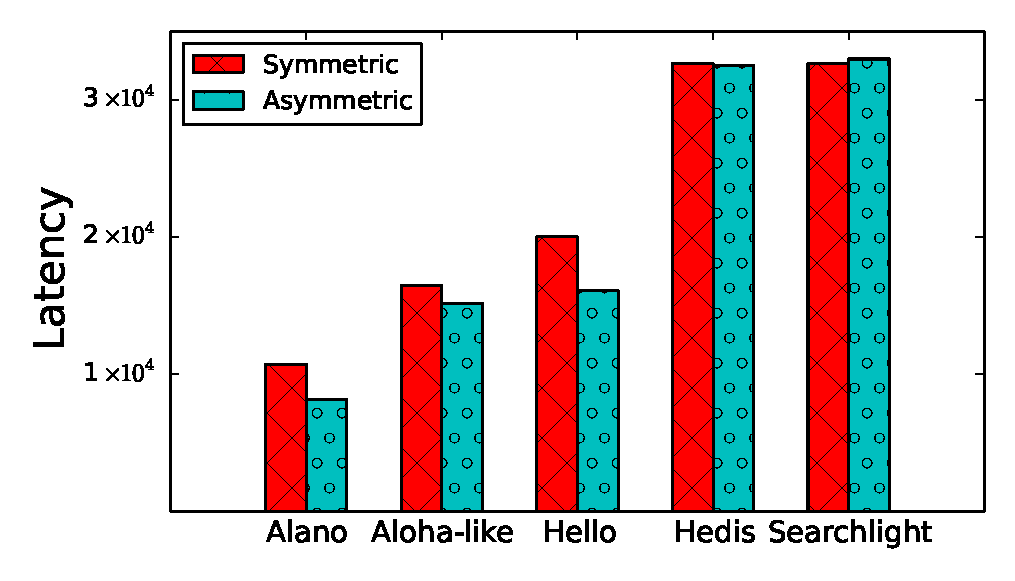
\includegraphics[width=1.65in]{Figure/latency_uniform}}
\hspace{0.01in}
\subfigure[Gaussian Distribution]{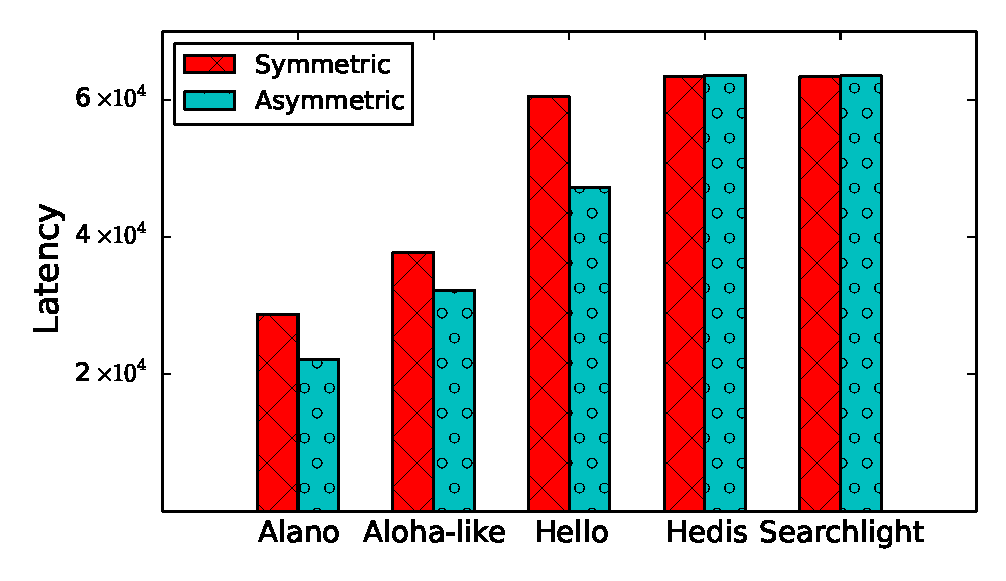
\includegraphics[width=1.65in]{Figure/latency_normal}}
\caption{Alano achieves $31.35\%$ to $2.91$ times lower latency.}
\label{fig_latency}
\end{figure}

When nodes follow uniform distribution, we show the discovery latency comparison for both symmetric nodes and asymmetric nodes in Fig. \ref{fig_latency}(a).
From the figure, Alano achieves $54.64\%$ to $1.95$ times lower discovery latency for symmetric nodes, and $85.25\%$ to $2.91$ times lower discovery latency for asymmetric nodes.
When nodes follow Gaussian distribution, as depicted in Fig. \ref{fig_latency}(b), 
Alano achieves $31.35\%$ to $1.21$ times lower discovery latency for symmetric nodes, 
and $45.94\%$ to $1.88$ times lower discovery latency for asymmetric nodes.
The deterministic algorithms, Hello, Hedis and Searchlight, have high latency due to either collisions or larger time slots. 


\subsubsection{Quality-Discovery Rate}

% \begin{figure}[!h]

% \subfigure[Uniform Distribution with Global Duty Cycle]{\includegraphics[width=1.65in]{Figure/rate_uniform}}
% \hspace{0.01in}
% \subfigure[Normal Distribution with Global Duty Cycle]{\includegraphics[width=1.65in]{Figure/rate_normal}}
% \hspace{0.01in}
% \subfigure[Uniform Distribution with Local Duty Cycle]{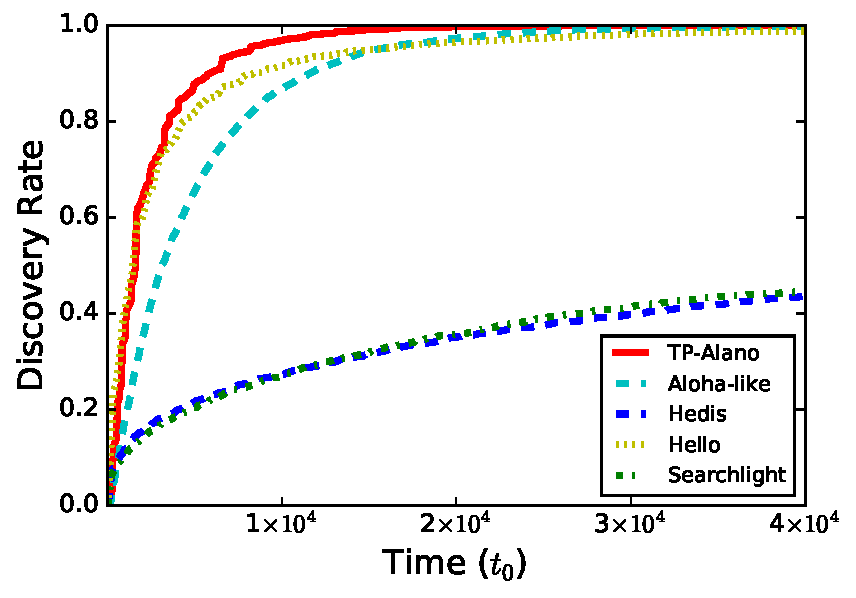
\includegraphics[width=1.65in]{Figure/rate_local_uniform}}
% \hspace{0.01in}
% \subfigure[Normal Distribution with Local Duty Cycle]{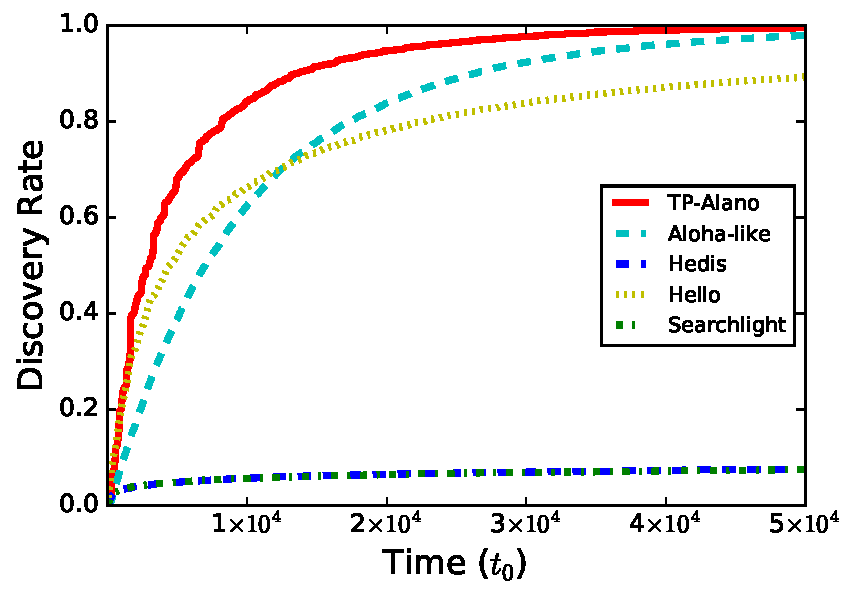
\includegraphics[width=1.65in]{Figure/rate_local_normal}}
% \caption{Alano achieves higher discovery rate.}
% \label{fig_timerate}
% \end{figure}


% Fig. \ref{fig_timerate} shows Alano with either global or local duty cycle, has higher discovery rate during the whole course of neighbor discovery in both uniform and normal distribution. The deterministic algorithms Hello, Hedis and Searchlight cannot discover all channels, because of the occurence of collisions. Aloha-like discovers more slowly than Alano when it has discovered a certain number of channels, such as $80\%$ channels in Uniform Distribution with Global Duty Cycle, because it is difficult for pure probabilistic algorithm to deal with the small amount of undiscovered neighbors.

\begin{figure}[!h]

\subfigure[Symmetric Nodes in Uniform Distribution]{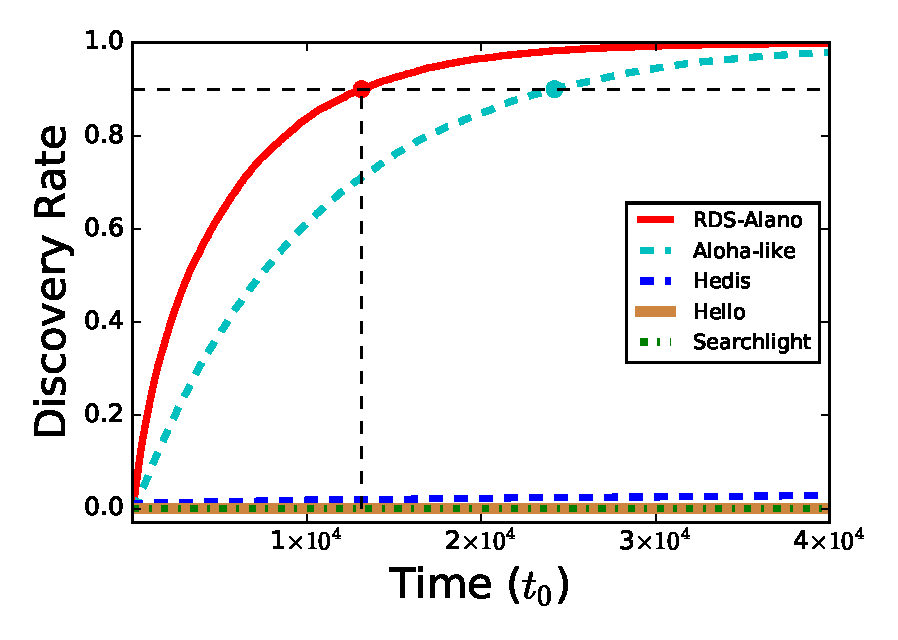
\includegraphics[width=1.65in]{Figure/rate_uniform1}}
\hspace{0.01in}
\subfigure[Symmetric Nodes in Gaussian Distribution]{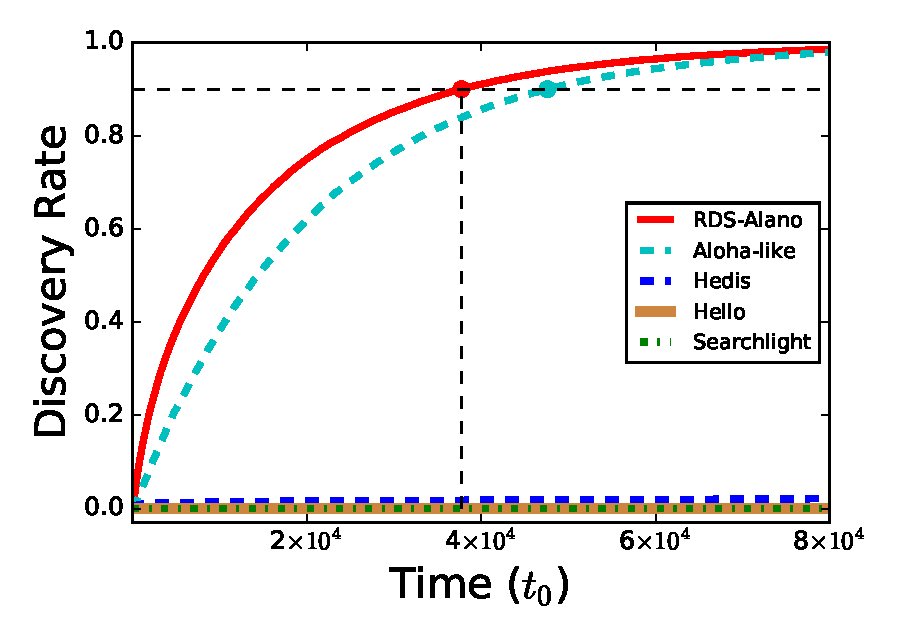
\includegraphics[width=1.65in]{Figure/rate_normal1}}
\hspace{0.01in}
\subfigure[Asymmetric Nodes in Uniform Distribution]{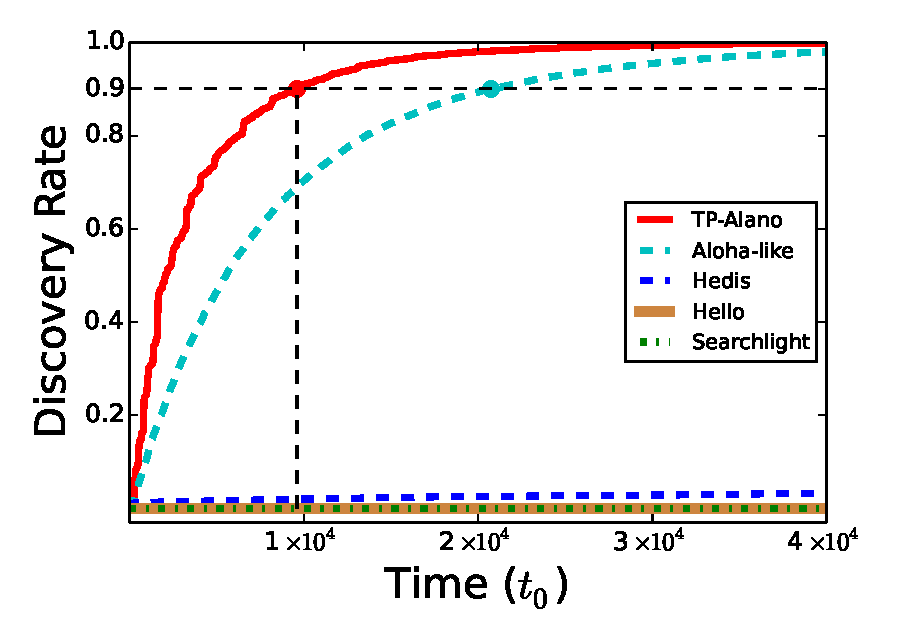
\includegraphics[width=1.65in]{Figure/rate_local_uniform1}}
\hspace{0.01in}
\subfigure[Asymmetric Nodes in Gaussian Distribution]{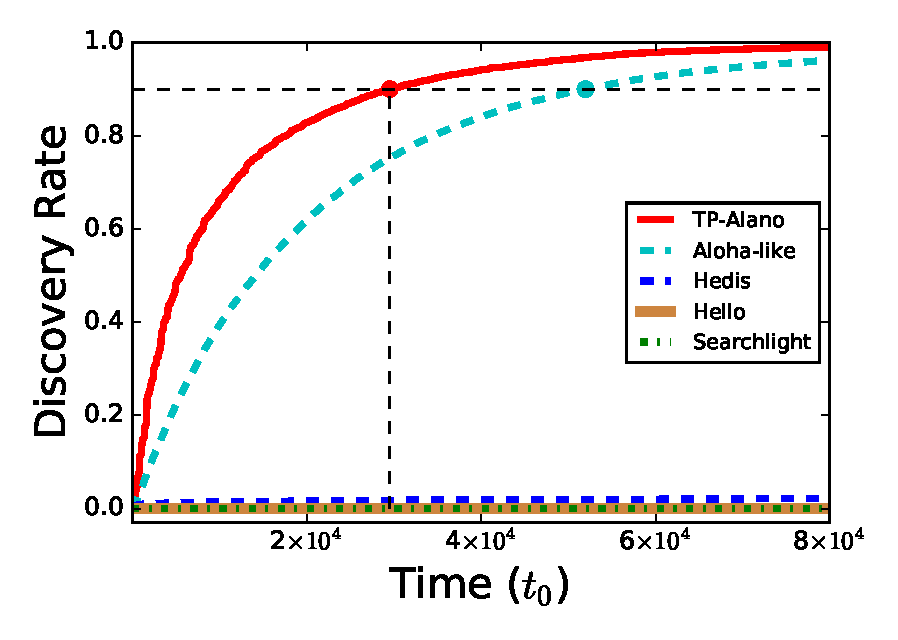
\includegraphics[width=1.65in]{Figure/rate_local_normal1}}
\caption{Alano has higher discovery rate during the whole process for both uniform and Gaussian distributions.}
\label{fig_timerate_large}
\end{figure}


We use discovery rate to evaluate Alano's quality.
Discovery rate of a node $u_i$ is defined as the percentage of discovered neighbors over $u_i$'s all neighbors.
In Fig. \ref{fig_timerate_large}, we increase the number of nodes from $500$ to $1000$ for the uniform distribution, and increase the number of nodes from $1000$ to $2000$ for the Gaussian distribution, the results show that Alano has higher discovery rate during the whole process for both uniform and Gaussian distributions. In the uniform distribution, Aano achieves 80\% discovery rate twice as fast as Aloha-like. It's remarkable that, the performance of Aloha-like is close to Alano in the Gaussian distribution. This is because a number of nodes gather around the center area which makes the network similar to a clique, and thus Aloha-like shows its strength.  
%Aloha-like discovers more slowly than Alano when it has discovered a certain number of channels, such as $80\%$ channels in Uniform Distribution with Global Duty Cycle, because it is difficult for pure probabilistic algorithm to deal with the small amount of  undiscovered neighbors.





\subsubsection{Scalability-Duty Cycle and Network Density}

We evaluated Alano's scalability regarding duty cycle and network density.

\begin{figure}[!h]
\centering
\subfigure[Uniform Distribution]{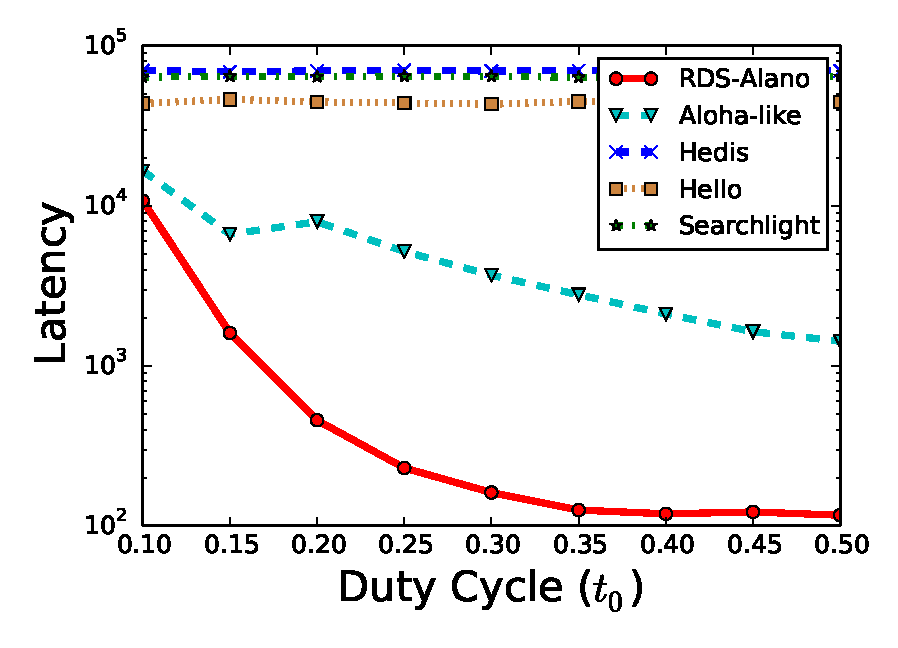
\includegraphics[width=1.65in]{Figure/dutycycle_uniform}}
\hspace{0.01in}
\subfigure[Gaussian Distribution]{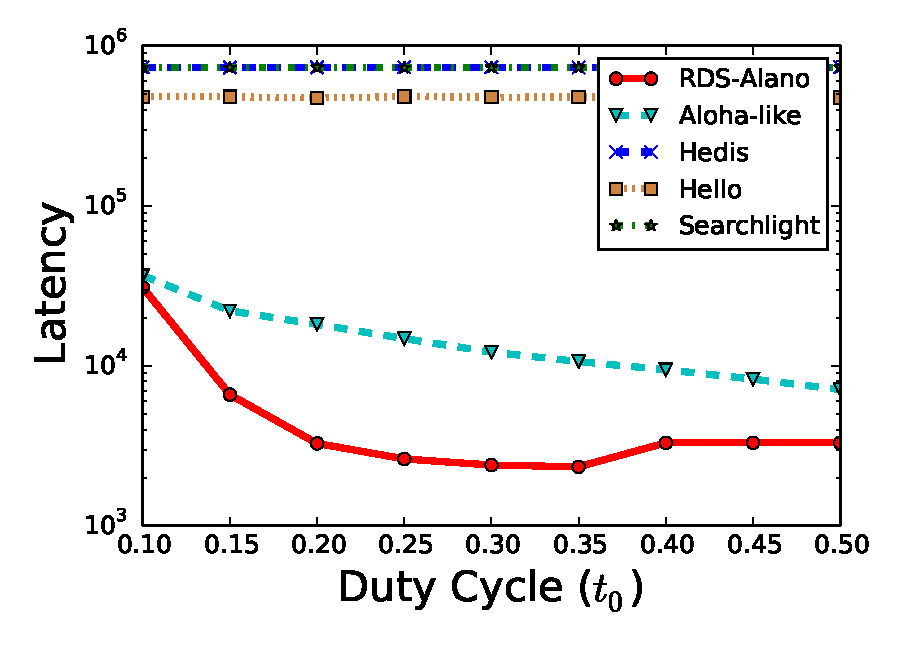
\includegraphics[width=1.65in]{Figure/dutycycle_normal}}
\caption{Alano achieves $53.66\%$ to $11.23$ times lower latency in different duty cycle.}
\label{fig_dutycycle}
\end{figure}


\emph{Duty Cycle.}
When symmetric nodes with different duty cycles, Fig. \ref{fig_dutycycle} shows that Alano has lower latency. Compared with Aloha, Alano has from $53.66\%$ to $11.23$ times lower latency. The latency of Alano and Aloha generally decreases as the duty cycle increases, while Hello, Hedis and Searchlight have high latency due to the collision. In Gaussian distribution, Alano has a small twist with duty cycle $0.35$, because when the duty cycle increases, nodes are more likely to transmit and therefore collide.


\begin{figure}[!h]
\centering
\subfigure[Uniform Distribution]{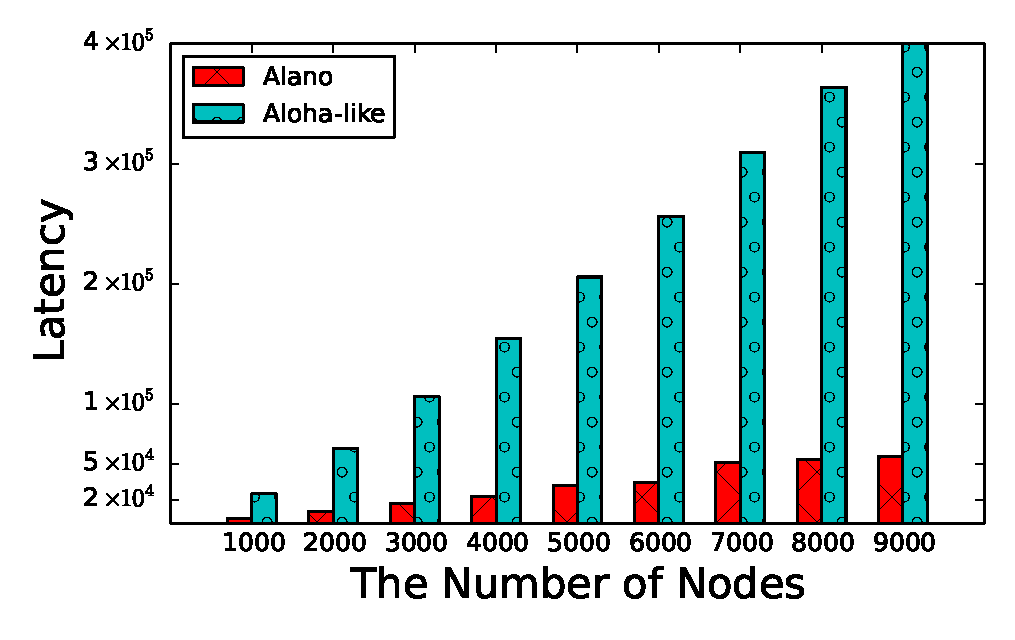
\includegraphics[width=1.65in]{Figure/node_uniform}}
\hspace{0.01in}
\subfigure[Gaussian Distribution]{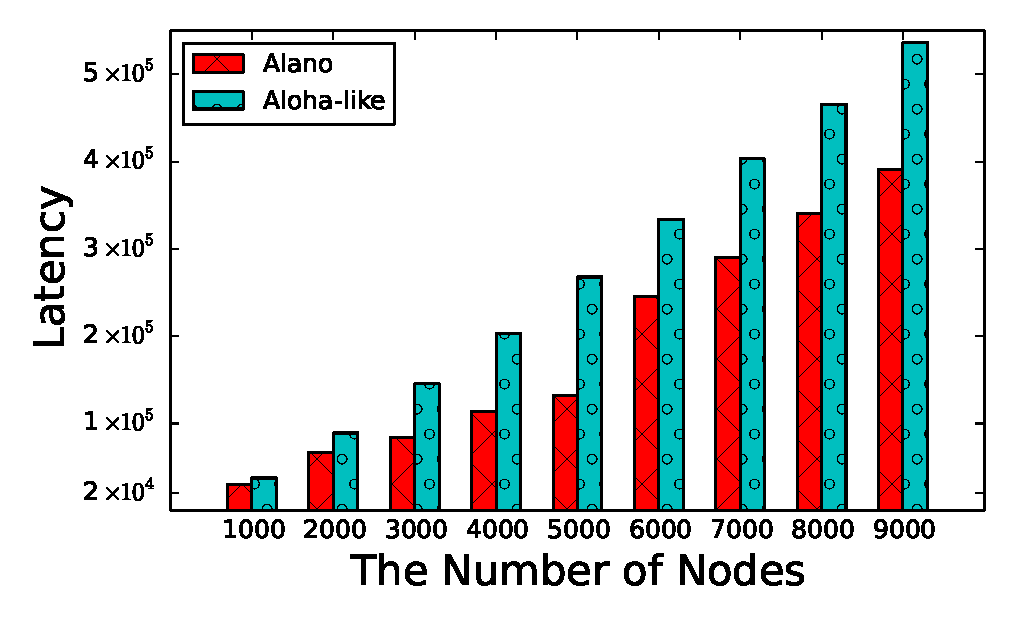
\includegraphics[width=1.65in]{Figure/node_normal}}
\caption{Alano achieves $25.23\%$ times to $6.51$ times lower latency when the network becomes denser.}
\label{fig_node}
\end{figure}

\emph{Network Density.}
When the number of nodes increases, the network becomes denser. We choose Aloha-like algorithm for comparison because Hello, Hedis and Searchlight already have higher latency than Aloha-like when there are $500$ nodes in uniform distribution and $1000$ nodes in Gaussian distribution.
As shown in Fig. \ref{fig_node}(a), Alano achieves $4.68$ times to $6.51$ times lower discovery latency than Aloha-like algorithm for uniform distribution, when the number of nodes increases from $1000$ to $9000$.
When the number of nodes increases from $1000$ to $9000$ for Gaussian distribution, Alano achieves $25.23\%$ to $1.03$ times lower discovery latency as shown in Fig. \ref{fig_node}(b).  

